One solution to the significant term mismatch between the query and the relevant documents is query expansion (QE)~\citep{Efthimiadis1996}, which has been effective in many retrieval tasks. The idea of QE is to add more terms to the original user's query to increase the probability of matching of the query terms with relevant documents, with the objective of improving retrieval effectiveness. The expansion terms can be selected from a feedback process or from external sources such as Wikipedia, or dictionaries~\citep{cao2008selecting}. Original queries should be expanded by good terms, unless it can lead to retrieval of irrelevant documents.
\paragraph{Feedback-based Query Expansion}
\ \\
An initial query can be expanded using a feedback from users --- relevance feedback --- or automatically from top $ k $ ranked retrieved documents, assuming they are relevant to the query --- pseudo relevance feedback (PRF)~\citep{manning2008introduction}. Getting feedback from  users needs user studies and interaction while pseudo relevance feedback is an automated process without user interaction.
\begin{figure}[t!]
%[htpb]
   \centering
   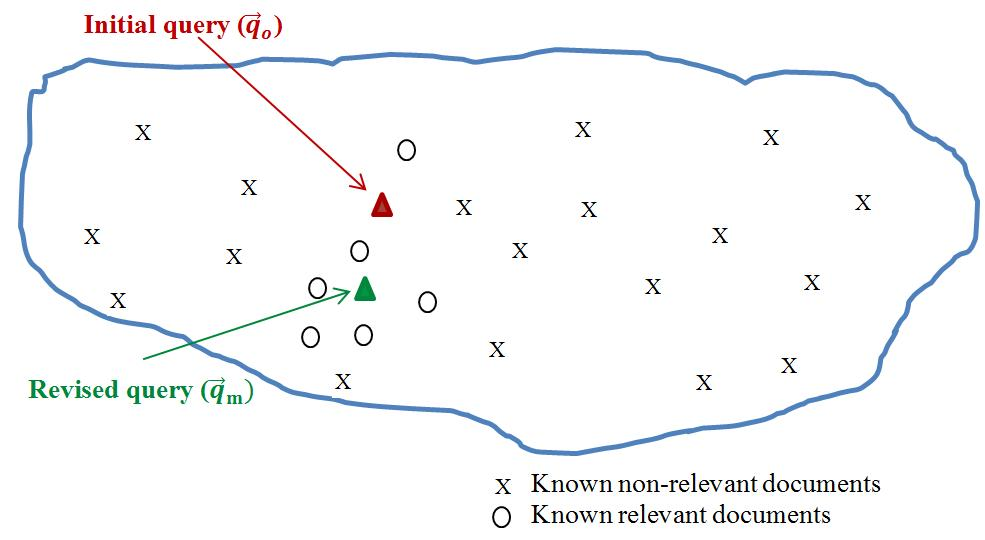
\includegraphics[width=0.65\textwidth,height=50mm]{figs/rocchio.jpg}
   \caption{Rocchio algorithm for relevance feedback. Some documents have been labelled as relevant and irrelevant and the initial query vector is moved in response to this feedback~\citep{manning2008introduction}.}  
   \label{fig:rocchio} 
\end{figure}
\FloatBarrier 
%\noindent
\textit{The Rocchio Algorithm for Relevance Feedback}: The Rocchio
algorithm \citep{Salton1971} is a classic algorithm of relevance feedback
used mainly for query expansion. In brief, it provides a method of
incorporating relevance feedback information into the vector space
model representing a query~\citep{manning2008introduction}. 
The rocchio algorithm is used to modify the query by the partial knowledge of known relevant and irrelevant~\footnote{In this thesis, we use irrelevant and non-relevant interchangeably for documents that are not relevant to the query.} documents; the goal is to move the query closer to the centroid of the relevant documents but further from irrelevant documents (Figure \ref{fig:rocchio}). The modified query $ \vec{q}_m $ is:
%\[ 
\begin{equation}
\label{eq:rocchio}
 \vec{q}_{m} = \alpha  \vec{q}_{0} + \beta\frac{1}{|D_{r}|}\sum\limits_{\vec{d_{j}}\in D_{r}} \vec{d_{j}} - \gamma\frac{1}{|D_{irr}|}\sum\limits_{\vec{d_{j}}\in D_{irr}} \vec{d_{j}},
  \end{equation}
 %\tag{2.1}\label{eq:rocchio}
 %\]  
where $ q_{0} $ is the original query vector; $ D_{r} $ and $ D_{irr} $ are the set of known relevant and irrelevant documents, respectively; and $ \alpha $, $ \beta $, and $ \gamma $ are weights attached to each term. These control the balance between trusting the judged document set versus the query: if we have a lot of judged documents, we
would like higher $ \beta $ and $ \gamma $~\citep{manning2008introduction}. 

PRF is typically used in Rocchio algorithm. However, it is important to distinguish between good expansion terms and bad ones. Distinguishing between expansion terms only based on their distribution in the feedback documents (i.e., extracting the most frequent terms) and in the whole collection (i.e., extracting the most specific terms) is not sufficient. It can be considered as a term classification problem to separate good expansion terms from others directly according to their potential impact on the retrieval effectiveness; hence, we can apply supervised learning methods for term selection. Classifiers like support vector machines (SVM)~\citep{cao2008selecting}, Na\"ive Bayes and Logistic Regression~\citep{he2009finding} can be used to classify terms and feedback documents.  
\paragraph{Query Expansion by External Resources}
\ \\
The most common form of query expansion is a global analysis, using dictionaries, WordNet, Wikipedia, or other thesaurus. For each term $ t $ in a query, the query can be automatically expanded with synonyms and related words of $ t $ from the thesaurus. Use of a thesaurus can be combined with ideas of term weighting; for instance, one might weight added terms less than original query terms~\citep{manning2008introduction}.